\chapter{Fluid flow around an elastic beam}

\modinfo{Directory}{FluiStructureBeam}
\modinfo{Solvers}{\Idx{ElasticSolve}, \Idx{FlowSolve}, \Idx{MeshSolve}}
\modinfo{Tools}{\Idx{ElmerGrid}, editor, \Idx{Fortran 90 compiler}}
\modinfo{Dimensions}{2D, steady-state}

\subsection*{Case definition}

A homogenous, elastic beam ($\Omega_2$) is in a fluid flow (which takes place
in the region $\Omega_1$), 
see figure~\ref{fg:fsi}. The beam is 5.0~m long and it is rigidly 
supported on the end $\Gamma_6$. At the incoming boundary $\Gamma_1$, the 
fluid velocity in the x-direction is a parabola which reaches its 
maximum value 1~m/s at the point y=5.0~m. At the incoming and outcoming 
boundaries $\Gamma_1$ and $\Gamma_2$ velocities in the y-direction 
are 0~m/s. At the outcoming boundary the pressure is 0~Pa. The velocities 
on boundaries $\Gamma_3$, $\Gamma_4$ and $\Gamma_5$ are 0~m/s. The 
fluid is incompressible and has density 1 kg/m$�$, dynamic 
viscosity 0.5 kg/ms and Poisson ratio 0.3. Material properties 
for the beam are the density 1000~kg/m$�$, Poisson ratio 0.3 and Young's 
modulus 1.0e3~N/m$�$. The problem is to solve the maximum displacement 
of the beam and the pressure change in $\Omega_1$.

\begin{figure}[h]
\centering
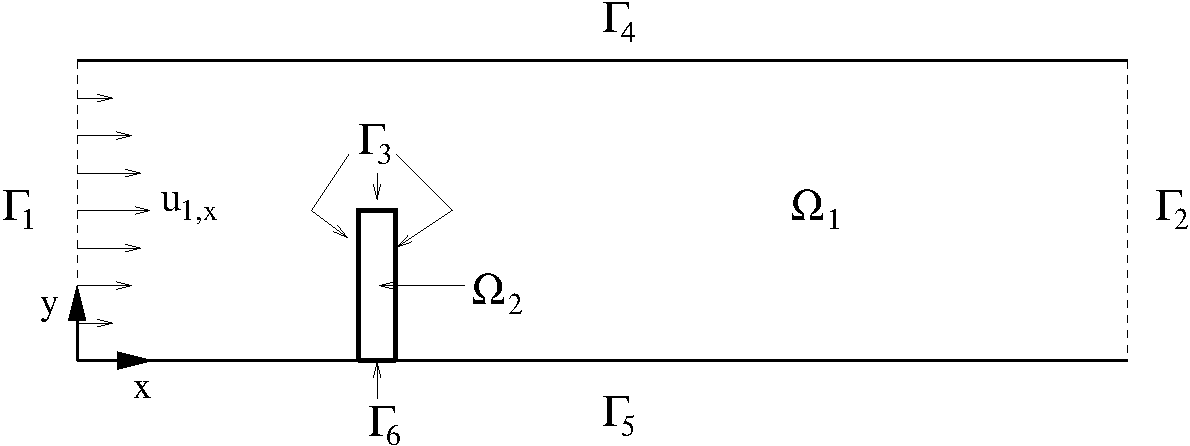
\includegraphics[width=100mm]{fsi}
\caption{Geometry of the problem}\label{fg:fsi}
\end{figure}

The flow generates normal and shear stresses to the beam
boundary $\Gamma_3$. These forces deform the beam and this changes the flow. 
This coupled problem can be modelled using the Navier-Stokes and elasticity 
equations. 

For the incompressible fluid the Navier-Stokes equations can be written as
\begin{equation}
\begin{array}{rcll}
- \nabla \cdot (2 \mu \overline{\overline{\varepsilon}}) + \rho 
\vec{u} \cdot \nabla \vec{u} + \nabla p &=& 0 & \mbox{ in } \Omega_1 \\
\nabla\cdot \vec{u}& = & 0 & \mbox{ in } \Omega_1 \\
\vec{u}_{x} &=& (10y-y^2)/25 & \mbox{ on } \Gamma_1 \\
\vec{u}_{x} &=& 0 & \mbox{ on } \Gamma_i ,\: i=3,4,5 \\
\vec{u}_{y} &=& 0 & \mbox{ on } \Gamma_i ,\: i=1,\ldots,5, 
\end{array}
\end{equation}
where $\mu$ is the dynamic viscosity, $\overline{\overline{\varepsilon}}$ is 
the strain tensor,  $\rho$ is the density, $\vec{u}$ is the velocity vector and
$p$ is the pressure. It is assumed that the density and viscosity are 
constants. 

For the homogeneous, elastic beam the elasticity equations are
\begin{equation}
\begin{array}{rcll}
-div [(I+ \nabla u) \Sigma] &=& 0 & \mbox{ in } \Omega_2 \\
\Sigma &=& \lambda (tr E)I + 2 \mu E & \mbox{ in } \Omega_2 \\
E &=& \frac{1}{2}(\nabla u^{T} + \nabla u + \nabla u^{T} \nabla u) 
& \mbox{ in } \Omega_2 \\
u &=& 0 & \mbox{ on } \Gamma_6 \\
(I+ \nabla u) \Sigma n &=& q & \mbox{ on } \Gamma_3 
\end{array}
\end{equation}
where $u$ is the displacement vector, $\Sigma$ is 
the second Piola-Kirchhoff stress tensor, $\lambda$ and $\mu$ are the Lam\'{e}
constants and $E$ is the Green-St Venant strain tensor, $q$ is the surface 
traction and $n$ is the unit normal to the beam boundary. The edge load $q$ is 
calculated from the stresses obtained using the Navier-Stokes equations.

For updating the fluids mesh a linear elasticity equation is used. In 
mathematical form it can be written as, 
\begin{equation}
\begin{array}{clcr}
-div \{\lambda tr [\varepsilon(v)]I + 2 \mu \varepsilon(v)\} = 0 & 
\mbox{ in } \Omega_1 \\
v = u_{\vert\Gamma_3} & \mbox{ on } \Gamma_3 \\
v = 0 & \mbox{ on } \Gamma_i, i=1,2,4,5 
\end{array}
\end{equation}
where $\lambda$ and $\mu$ are the Lam\'{e} constants, $\varepsilon$ is
linear strain tensor and $v$ is the displacement vector. Here $u$ is the 
solution to the elasticity equations.


\subsection*{Solution procedure}

In this problem geometry and mesh is created by using ElmerGrid by the 
command
\ttbegin
ElmerGrid 1 2 fsi.grd
\ttend

In this problem, external Fortran functions are used to express a
parabolic velocity inflow profile and to define a variable stiffness
for the deforming mesh. The stiffness of the mesh is controlled by the
Youngs modulus. In the case of deforming mesh, the absolute value of
the parameter is not important but its changes over the domain are
influential. The following function defines the mesh to be stiffer
near the corner of the beam where the mesh is deformed most. The idea
is to avoid too irregularly shaped elements in that area.

\ttbegin
FUNCTION Youngs( Model, n, x ) RESULT( s )
  USE Types
  IMPLICIT NONE

  TYPE(Model_t) :: Model
  INTEGER :: n
  REAL(KIND=dp) :: x,s,xx,yy
  
  xx = Model % Nodes % x(n)
  yy = Model % Nodes % y(n)
  
  s =  1.0d0 / SQRT( (xx-11.0)**2 + (yy-4.9)**2 )
  
END FUNCTION Youngs
\ttend

The following function is used to give the inflow boundary condition.

\ttbegin
FUNCTION InFlow( Model, n, x ) RESULT( vin )
  USE Types
  IMPLICIT NONE

  TYPE(Model_t) :: Model
  INTEGER :: n
  REAL(KIND=dp) :: yy,xx,x,vin,v0,vt

  xx = Model % Nodes % x(n)
  yy = Model % Nodes % y(n)
  
  v0 = (-(yy**2)+10*yy)/25
  
  IF(x < 8.0) THEN
    vt = x/8.0
  ELSE
    vt = 1.0
  END IF

  vin = v0*vt

END FUNCTION InFlow
\ttend

In general, the user may supply his/hers own functions for defining
general dependencies of variables or parameters. The function header
should read as follows
\ttbegin
FUNCTION FunctionName( Model, n, x ) RESULT( res )
\ttend
where {\tt Model} is a structure holding various information�of the
problem and {\tt n} is the number of the node being considered. These
are automatically given by the program. The paramter {\tt x} is the
value of the variable, which user defines to be given for the function
as input. The variable is defined in the sif file. Finally, a the
function returns the result {\tt res} for the parameter in
consideration. 

If the Elmer environment is succesfully setup the compilation command 
should look like
\ttbegin
elmerf90 -o FsiStuff FsiStuff.f90
\ttend

The functions may be compiled also locally on a PC either for Linux or
WindowsNT, provided that a Fortran90 compiler and the Elmer software
are installed.

The next step is to edit the solver input file (\texttt{sif} file)
with a text editor, {\em e.g.} Emacs.
\begin{itemize}
\item The Header section, where the mesh is defined. 
%
\ttbegin
Header 
  Mesh DB "." "fsi" 
End
\ttend
%
\item The \texttt{Constants} section need not contain any constant this time.
%
\ttbegin
Constants
End
\ttend
%
\item The \texttt{Simulation} section gives the control data for the case.
%
\ttbegin
Simulation
  Coordinate System = Cartesian 2D
  Simulation Type = Steady State
  Steady State Max Iterations = 50
  Steady State Min Iterations = 2
  Output Intervals = 1
  Output File = "fsi.result"
  Post File = "fsi.ep"
End
\ttend
%
\item The \texttt{Body} section is used to define which equations and
materials are used for the simulation bodies.
($\Omega_2$).
%
\ttbegin
Body 1
  Equation = 1
  Material = 1
End

Body 2 
  Equation = 2 
  Material = 2 
End
\ttend
%
\item The \texttt{Material} section defines the material properties of
each body. Also the procedure \texttt{Youngs} is used. 
%
\ttbegin
Material 1 
  Density = 1.0 
  Viscosity = 0.5 
  Poisson Ratio = 0.3 
  Youngs Modulus = Variable time 
      Real Procedure "FsiStuff" "Youngs" 
End

Material 2
   Density = 1000
   Youngs Modulus = 1.0e3
   Poisson Ratio = 0.3
End
\ttend
%
\item The Solver section defines various control parameters for each 
solver.
%
\ttbegin
Solver 1
  Equation = Navier-Stokes
  Stabilize = True
  Linear System Solver = Iterative
  Linear System Iterative Method = BiCGStab
  Linear System Preconditioning = ILU1
  Linear System Max Iterations = 500
  Linear System Convergence Tolerance = 1.0e-8
  Nonlinear System Max Iterations = 10
  Nonlinear System Convergence Tolerance = 1.0e-5
  Nonlinear System Newton After Tolerance = 1.0e-5
  Nonlinear System Newton After Iterations = 20
  Nonlinear System Relaxation Factor = 1.0
  Steady State Convergence Tolerance = 1.0e-4
End

Solver 2
  Equation = Elasticity Solver
  Variable = Displacement
  Variable DOFs = 2
  Procedure = "ElasticSolve" "ElasticSolver"
  Linear System Solver = Direct
  Linear System Direct Method = Banded
  Nonlinear System Newton After Tolerance = 1.0e-3
  Nonlinear System Newton After Iterations = 20
  Nonlinear System Max Iterations = 100
  Nonlinear System Convergence Tolerance = 1.0e-5
  Nonlinear System Relaxation Factor = 1.0
  Steady State Convergence Tolerance = 1.0e-4
End

Solver 3 
  Equation = Mesh Update
  Linear System Solver = Iterative
  Linear System Iterative Method = BiCGStab
  Linear System Preconditioning = ILU1
  Linear System Max Iterations = 500
  Linear System Convergence Tolerance = 1.0e-8
  Steady State Convergence Tolerance = 1.0e-4
End
\ttend
%
\item The \texttt{Equation} section. This section defines the
equations for a body. Plane stress model for the elastic beam is 
applied. Setting this keyword to {\tt False} enables the plane 
strain assumption.
%
\ttbegin
Equation 1
  Active Solvers(2) = 1 3
End

Equation 2
  Active Solvers = 2
  Plane Stress = True
End
\ttend
%
\item In the \texttt{Boundary Condition} section different boundary
conditions are defined.  In Boundary Condition~1 the shape of inflow
is defined with the Fortran procedure \texttt{InFlow}. Note also the
bc 3, where keyword {\tt FSI BC} is supplied to define the boundary on
which the fluid affects a force on the elastic beam. Also, on the same
boundary, the mesh is constraint to follow the deformation of the beam
by the two Equals lines.
%
\ttbegin
Boundary Condition 1 
  Target Boundaries = 1
  Velocity 1 = Variable Time
      Real Procedure "FsiStuff" "InFlow"

  Velocity 2 = 0.0
  Mesh Update 1 = 0.0
End 

Boundary Condition 2
  Target Boundaries = 2
  Velocity 2 = 0.0
  Pressure = 0.0
  Mesh Update 1 = 0.0
End

Boundary Condition 3 
  Target Boundaries = 3
  Velocity 1 = 0.0
  Velocity 2 = 0.0
  FSI BC = True
  Mesh Update 1 = Equals Displacement 1
  Mesh Update 2 = Equals Displacement 2
End

Boundary Condition 4
  Target Boundaries(2) = 4 5
  Velocity 1 = 0.0
  Velocity 2 = 0.0
  Mesh Update 2 = 0.0
End

Boundary Condition 5
  Target Boundaries = 6 
  Displacement 1 = 0.0
  Displacement 2 = 0.0
End
\ttend
%
\end{itemize}

\subsection*{Results}

After the solution is done, view the results with ElmerPost. 
Read the result file fsi.ep in ElmerPost by choosing Read Model File. The 
fsi.ep file is located in the same directory as the mesh files. 

\begin{table}[tbhp]
\caption{Max. displacement and pressure difference}
\label{tb:struct5}
\begin{center}
\begin{tabular}{lll} \hline
Elements & $\max |u|$ [m] & $\max \Delta p$ [Pa] \\  \hline 
540  &  1.34  &  6.36  \\ \hline 
\end{tabular}
\end{center}
\end{table}

As a result the maximum absolute value of displacement and the 
pressure difference is given (see table~\ref{tb:struct5}).
